\section{Theory}
% Delaunay-triangulering, punktsett, sirkelkriterie, distmesh (ikke 3D), etc.
To produce and use grid representations of the real world, there must be a way to map the real, continuous domain to a discrete representation. This is typically done by looking at a set of points in the real domain.

\begin{definition}[Point set]
A point set $P \in \mathbb{R}^n$ is a finite set of points in $\mathbb{R}^n$.
\end{definition}
While there exists infinite point sets, we limit ourselves to finite sets in order to be have a discrete representation. In order to encode more data in the discrete representation, points in a point set can be grouped in simplices. This enables the inclusion of data about physical properties such as subsurface faults, wells and other geological features, which are necessary for accurate simulations. Using simplices to represent a domain allows us to reduce the amount of data necessary for representing a domain with physical features, compared to using a large point set to represent the domain.


\begin{definition}[Simplex]
A simplex is a generalization of a triangle to arbitrary dimensions.
\end{definition}
Simplices represent the simplest possible geometric object in a space. As grid representations of real scenarios are limited to three dimensions, we only need to consider the first four simplices:
\begin{itemize}
    \item A 0-simplex is a point,
    \item A 1-simplex is a line,
    \item A 2-simplex is a triangle,
    \item A 3-simplex is a tetrahedron.
\end{itemize}

\begin{figure}[ht]
    \centering
    \begin{subfigure}[b]{0.2\textwidth}
        \centering
        
\includegraphics[width=\textwidth]{report/Images/Theory/simplices/simplices0.png}
        \caption{0-simplex}
        \label{fig:0-simplex}
    \end{subfigure}
    \hfill
    \begin{subfigure}[b]{0.2\textwidth}
        \centering
        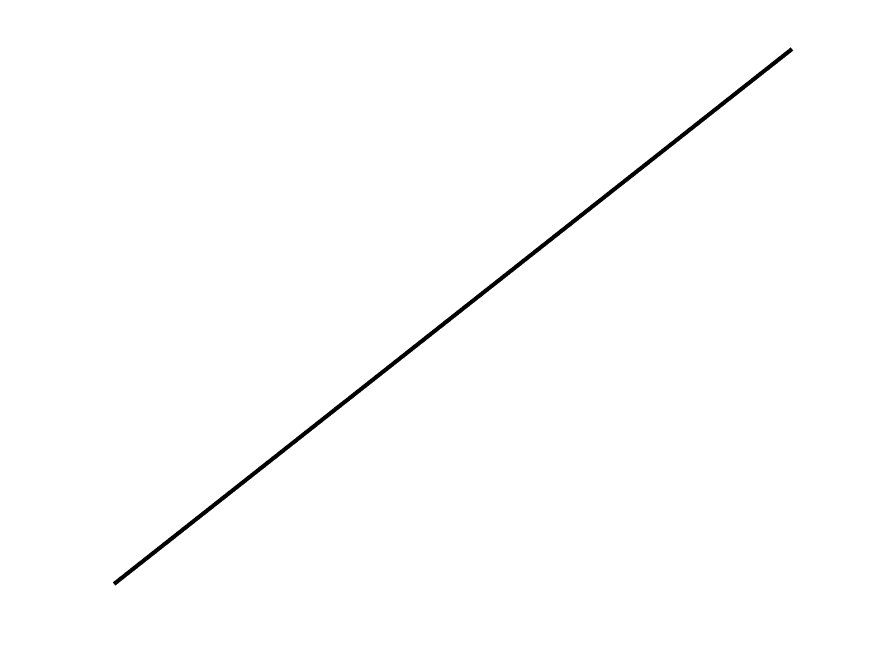
\includegraphics[width=\textwidth]{report/Images/Theory/simplices/simplices1.png}
        \caption{1-simplex}
        \label{fig:1-simplex}
    \end{subfigure}
    \hfill
    \begin{subfigure}[b]{0.2\textwidth}
        \centering
        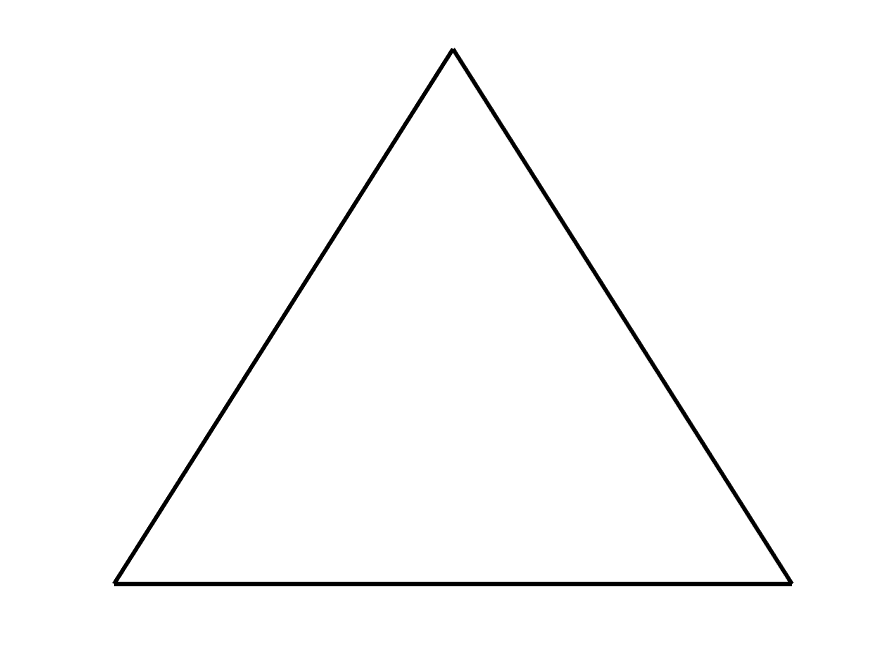
\includegraphics[width=\textwidth]{report/Images/Theory/simplices/simplices2.png}
        \caption{2-simplex}
        \label{fig:2-simplex}
    \end{subfigure}
    \hfill
    \begin{subfigure}[b]{0.2\textwidth}
        \centering
        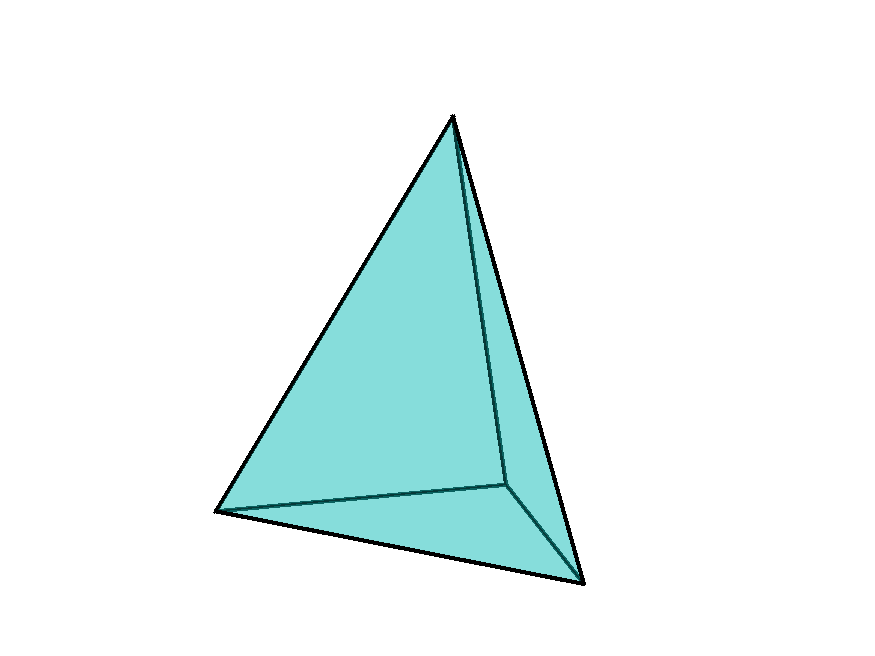
\includegraphics[width=\textwidth]{report/Images/Theory/simplices/simplices3.png}
        \caption{3-simplex}
        \label{fig:3-simplex}
    \end{subfigure}
    \hfill
    \caption{Illustration of the first 4 simplices}
    \label{fig:simplices}
\end{figure}

In general, a $k$-simplex is a $k$-dimensional geometric object consisting of the \emph{convex hull} of its $k + 1$ vertices.


\begin{definition}[Convex hull]
The convex hull of a point set $P$ is the minimal convex set containing $P$.
\end{definition}
\begin{figure}[ht]
    \centering
    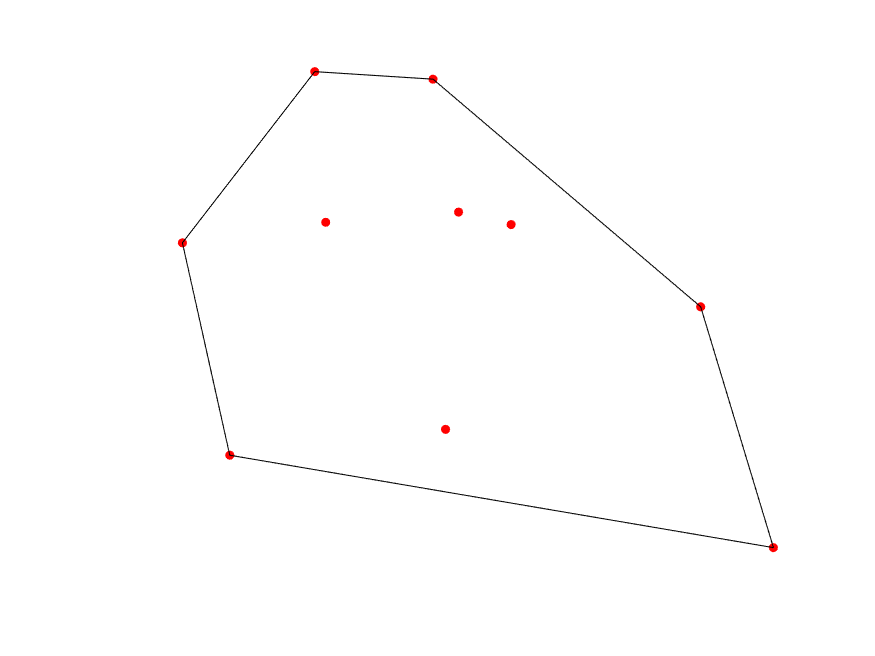
\includegraphics[width=0.5\textwidth]{report/Images/Theory/convex_hull.png}
    \caption[Example of a convex hull]{Example of a convex hull for a set of 10 randomly generated points in $\mathbb{R}^2$.}
    \label{fig:ex:convex_hull}
\end{figure}

The process of converting a point set into a set of simplices is called \emph{triangulation}.

\begin{definition}[Triangulation]
A triangulation $T$ of a point set $P$ is the set of simplices $T$ such that
\begin{itemize}
    \item The set of vertices in $T$ equals $P$
    \item The union of all simplices in $T$ equals the convex hull of $P$, i.e. the union of all simplices in $T$ makes up the minimal convex set containing $P$.
\end{itemize}
\end{definition}
\begin{figure}[ht]
    \centering
    \begin{subfigure}[b]{0.4\textwidth}
        \centering
        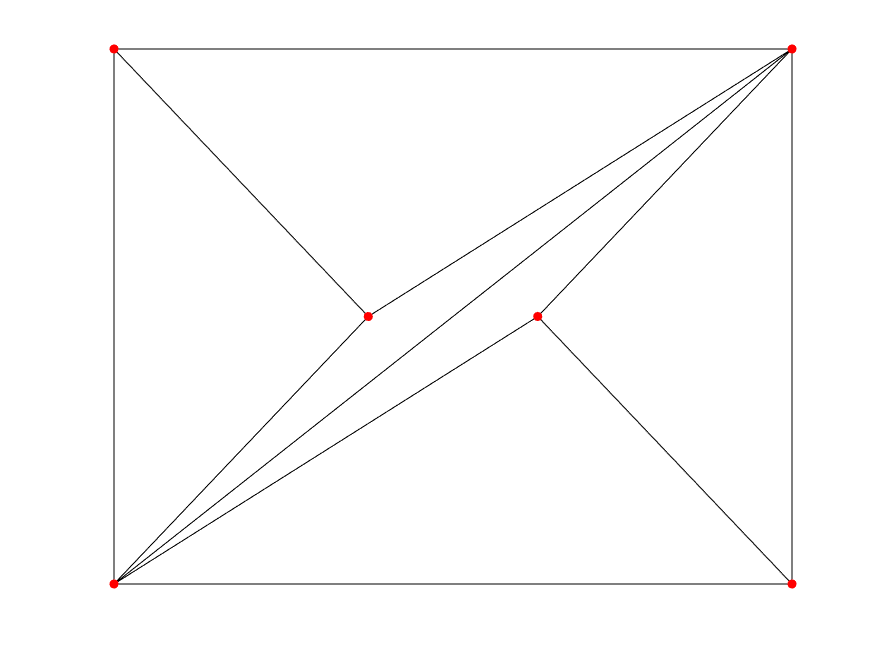
\includegraphics[width=\textwidth]{report/Images/Theory/triangulation/triangulation_random.png}
        \caption{Random triangulation}
        \label{fig:triangulation-random}
    \end{subfigure}
    \begin{subfigure}[b]{0.4\textwidth}
        \centering
        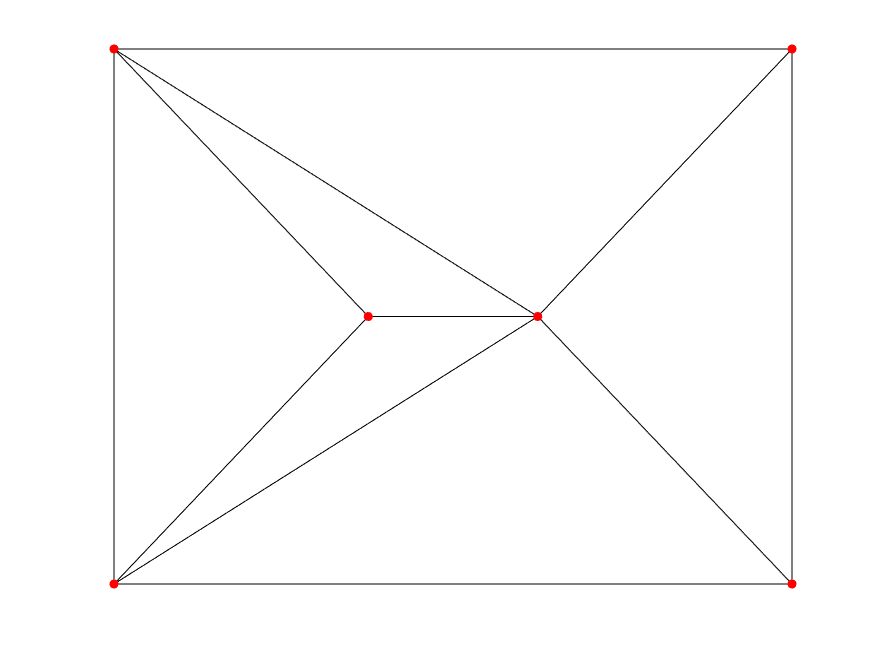
\includegraphics[width=\textwidth]{report/Images/Theory/triangulation/triangulation_delaunay.png}
        \caption{Delaunay triangulation}
        \label{fig:triangulation-delaunay}
    \end{subfigure}
    \caption[Example of triangulation]{Example of two triangulations for a set of points $P \in \mathbb{R}^2$.}
    \label{fig:ex:triangulation}
\end{figure}

For a given point set, one can generally create multiple legal triangulations. \autoref{fig:ex:triangulation} shows two triangulations for the same point set $P$.


\subsection{Delaunay triangulation}
Delaunay triangulation is a triangulation first introduced by \textcite{delaunay_1943} in 1943. Delaunay triangulations maximize the smallest angle of the simplices in the triangulation, and therefore produce representations that work nicely in grid-based applications. The Delaunay triangulation of a point set $P$ is defined as follows:
\begin{definition}
Let $T$ be a triangulation of the point set $P$. $T$ is a Delaunay triangulation if no vertices in $P$ are inside the \emph{circumcircle} of any simplex in $T$.
\end{definition}

\begin{definition}[Circumcircle]
A circumcircle of a polygon is a circle passing through all vertices of the polygon. The circumcircles of a triangulation is the set of circumcircles of all simplices in the triangulation.
\end{definition}

\begin{figure}[ht]
    \centering
    \begin{subfigure}[b]{0.4\textwidth}
        \centering
        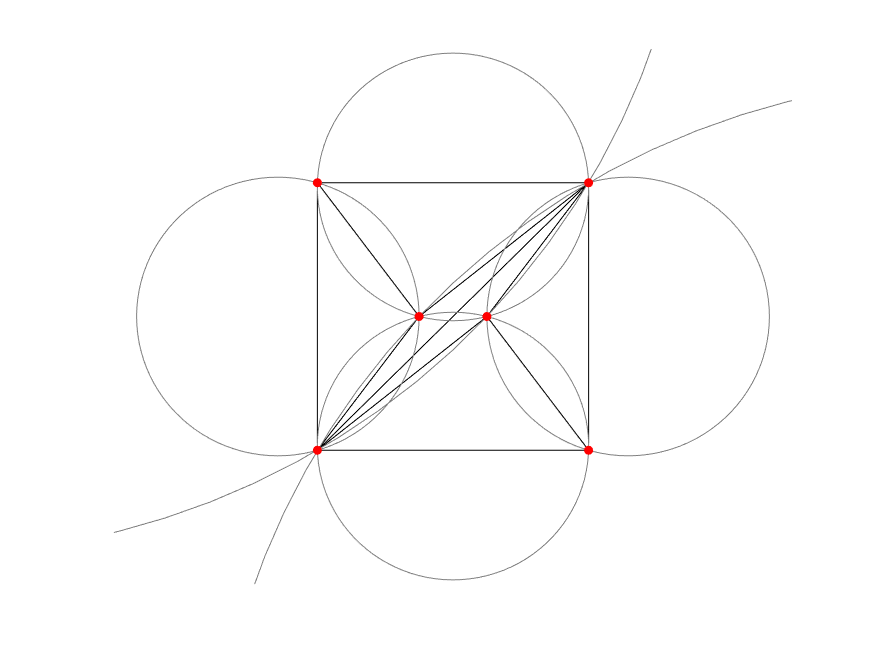
\includegraphics[width=\textwidth]{report/Images/Theory/circumcircles/circumcircle_random.png}
        \caption{Circumcircles of \autoref{fig:triangulation-random}}
        \label{fig:circumcircles-random}
    \end{subfigure}
    \begin{subfigure}[b]{0.4\textwidth}
        \centering
        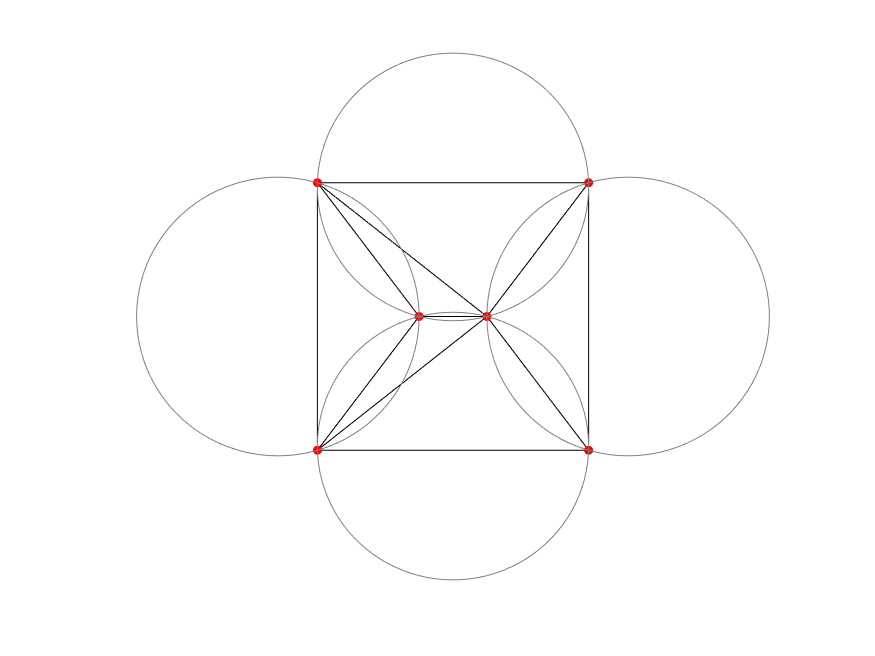
\includegraphics[width=\textwidth]{report/Images/Theory/circumcircles/circumcircle_delaunay.png}
        \caption{Circumcircles of \autoref{fig:triangulation-delaunay}}
        \label{fig:circumcircles-delaunay}
    \end{subfigure}
    \caption[Example of circumcircles]{Example of circumcircles for the two triangulations in \autoref{fig:ex:triangulation}. Note that \autoref{fig:circumcircles-random} has a been cropped.}
    \label{fig:ex:circumcircles}
\end{figure}


In \autoref{fig:circumcircles-delaunay}, no vertices of $P$ are inside any of the plotted circumcircles. This shows that the triangulation in \autoref{fig:triangulation-delaunay} is a Delaunay triangulation. In \autoref{fig:circumcircles-random}, two vertices are inside each of the two large circumcircles created from the centermost, narrow triangles. This shows that the triangulation in \autoref{fig:triangulation-random} is not Delaunay.

Delaunay triangulations are unique as long as at most three vertices are on the same circumcircle. In cases where this is not true, such as where four vertices make up a cyclic quadrilateral, there exist several legal Delaunay triangulations for the same point set $P$. This is illustrated in \autoref{fig:non-unique-delaunay}, where the two center vertices make up cyclic quadrilaterals with both the top and bottom pair of vertices. This enables four legal Delaunay triangulations of the point set.

\begin{figure}[ht]
    \centering
    \begin{subfigure}[t]{0.4\textwidth}
        \centering
        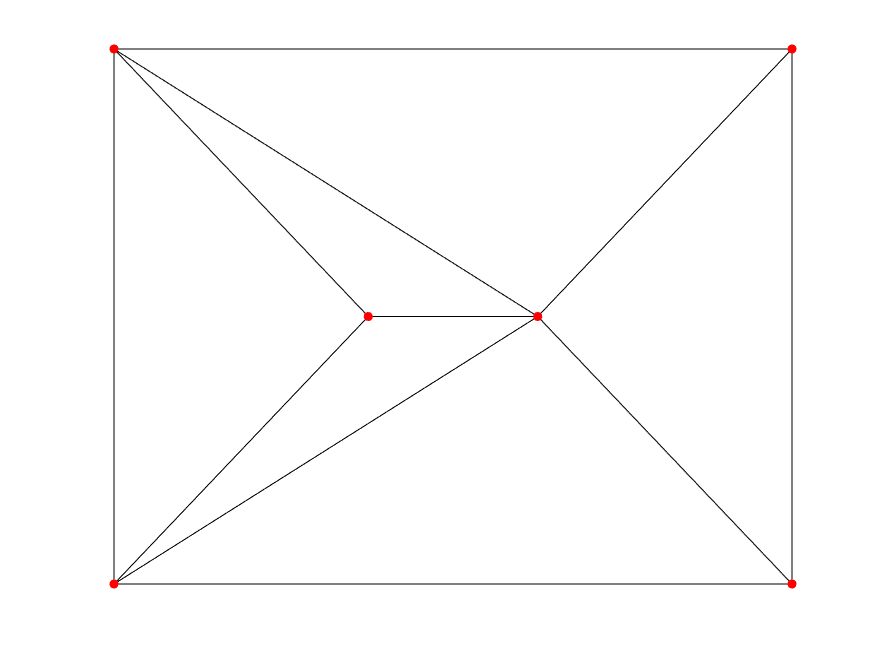
\includegraphics[width=\textwidth]{report/Images/Theory/triangulation/triangulation_delaunay.png}
        \label{fig:triangulation-delaunay1}
    \end{subfigure}
    \begin{subfigure}[t]{0.4\textwidth}
        \centering
        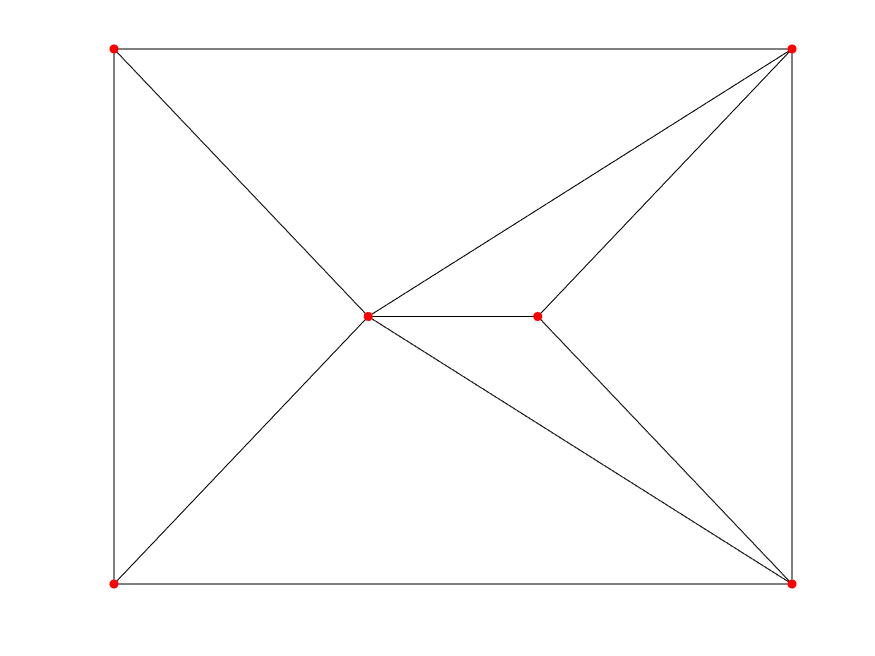
\includegraphics[width=\textwidth]{report/Images/Theory/triangulation/triangulation_delaunay2.png}
        \label{fig:triangulation-delaunay2}
    \end{subfigure}
    \begin{subfigure}[b]{0.4\textwidth}
        \centering
        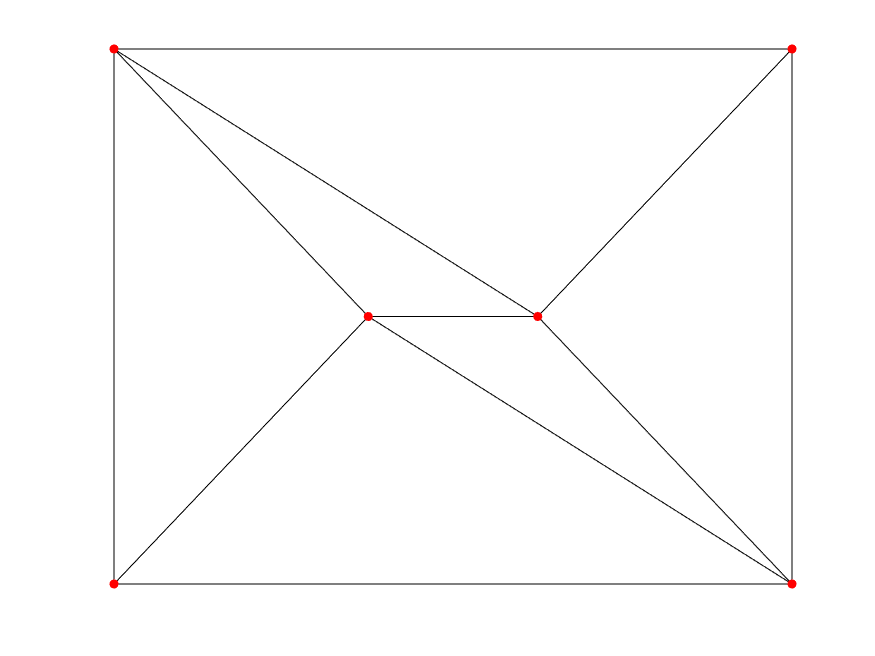
\includegraphics[width=\textwidth]{report/Images/Theory/triangulation/triangulation_delaunay3.png}
        \label{fig:triangulation-delaunay3}
    \end{subfigure}
    \begin{subfigure}[b]{0.4\textwidth}
        \centering
        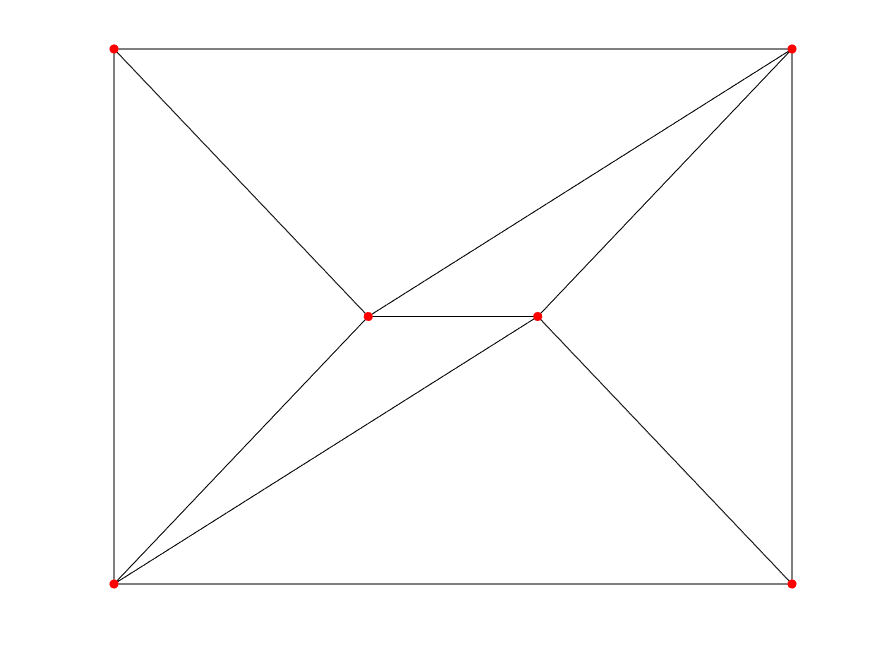
\includegraphics[width=\textwidth]{report/Images/Theory/triangulation/triangulation_delaunay4.png}
        \label{fig:triangulation-delaunay4}
    \end{subfigure}
    \caption[Non-uniqueness of Delaunay triangulations]{Non-uniqueness of Delaunay triangulations. Two cyclic quadrilaterals enables four legal Delaunay triangulations.}
    \label{fig:non-unique-delaunay}
\end{figure}



\subsection{Voronoi diagrams}


\subsection{Distmesh}

\subsection{PEBI grids}
\textcolor{red}{DETTE ER IKKE FERDIG}

\begin{equation}
    v_{s_i} = \left\{ x : x \in \mathbb{R}^d,\quad \abs{x - s_i} < \abs{x - s},\quad \forall s \in S \setminus \{s_i\} \right\}.
\end{equation}
The face between two sites, denoted by $v_{s_i, s_j}$ is made up by all points that are the same distant from two sites but further from any other sites, i.e.
\begin{equation}
    v_{s_i, s_j} = \left\{ x : x \in \mathbb{R}^d,\quad \abs{x - s_i} = \abs{x - s_j} < \abs{x - s},\quad \forall s \in S \setminus \{i, j\} \right\}.
\end{equation}

% Legg til en illustrasjon av PEBI